\documentclass[10pt]{article}
\usepackage{hyperref}
\usepackage{graphicx}
%opening
\title{Personal Statement and Summary of Accomplishments}
\author{Andrew Rosen\\Assistant Professor of Instruction}
\date{}

\begin{document}

\maketitle


\section{Preface}
This document serves as a overview of my accomplishments thus far at Temple University.  
I came to Temple in the Fall of 2016.
I was hired as an Assistant Professor of Instruction because of my record of teaching excellence and remarkable amount of experience, having taught numerous courses solo as a PhD student.
I have proven myself to be an exceptional teacher, as demonstrated by being awarded the Dean's Distinguished Teaching Award in the Fall of 2018.

I teach CIS 1051 -  Introduction to Problem Solving and Programming in Python - and have taught CIS 1068 -  Program Design and \& Abstraction, both of which serve as introductory courses to computer science.
CIS 1051 is an extremely large course, with over 140 students, with a variety of students of differing skill levels, background experience, and majors.
I also teach CIS 2168 - Data Structures,  which serves as prerequisite to almost all upper level classes in computer science and is one of the courses large tech companies look at when evaluating and interviewing students.
Coporations such as Google, Microsoft, Amazon, and Apple all look at student's performance in Data Structures when evaluating candidates and  interview problems are nearly guaranteed to draw from the concepts in this class.  
I also have served as the course coordinator for CIS 2168 since the fall of 2018, writing the common final and coordinating the material to be taught between sections.
Finally, I have developed and teach a new online graduate course, CIS 5016 - Data Structures and Objects.
%These classes expose me to a great variety of students and can be quite challenging to accommodate the skill disparity often seen in Computer Science courses.

What distinguishes me as a Professor is dedication constant improvement of my courses and making as great of an experience for my students as possible.
I am always willing to go that extra mile for my students and to improve our department's curriculum.
My accomplishments and reasons for promotion are:

\begin{itemize}
	\item I was the recipient of the 2018 Dean’s Distinguished Teaching award for my excellence in teaching.
	\item I became the first faculty member to teach Computer Science courses at Temple University Japan and setup the courses to be run on campus locally for the first  time.  I gave the faculty there the tools to continue to provide Computer Science courses locally at TUJ, with our eventual goal is to offer a Computer Science minor that can be completed solely at the Japan campus.
	
	\item I find and develop assignments that are engaging to our students, build a portfolio for students to show prospective employers, and develop the skills they need to succeed in the industry.
	
	\item I have become the leading faculty member in my department to ``flip'' a classroom, which has students watch lectures before coming to class, where they work on assignments and other active learning exercises.
	\item My student feedback forms show repeatedly high evaluations from students, scoring a 4.9 and 5.0 in my most recent semesters in ``I learned a great in this course'' and ``The instructor taught this course well.''  My students continually report that the assignments I develop, the techniques I use, the novel approaches I use to teach my course, the care I show and  accommodations make for them overwhelmingly to better outcomes. 

	 
	\item I have  developed a new course for graduate students in our Masters in IST program, which is designed to transition a student with very little programming experience to a student who is ready for graduate level coursework.
	\item I am one of the two initial faculty members in our department to develop and teach an online course.
	\item I have been working with the Office of Digital Education to create high quality videos for our online courses that can also be fed back into our undergraduate courses.  An example video can be found here: \url{https://player.vimeo.com/video/313364524}
	\item I have attended a number of workshops to further my teaching skills and to learn how to improve my course.  I have also attended SIGCSE as part of furthering my teaching skills.
	\item I am mentoring other faculty members on how to develop online courses and create effective recorded lectures for programming courses.
	\item I have taken over the responsibilities of coordinating faculty  and creating the common  final exam for teaching CIS 2168.
	\item Students find me approachable and consistently come in for my office hours.  I also make sure I can meet students who need additional help or can't make it to normal office hours due to work or class conflicts by  meeting via video chat program.   I have seen many instances where this late night instruction over video chat has made a concept ``click'' for a student.
\end{itemize}

%Computing is a field that is in high demand right now, and students who successfully complete their degree are able to command extremely high salaries

These all demonstrate that I am a highly skilled and effective teacher who is always looking for a way to improve upon what we can offer our students. I am always willing to step forward and be the first to try something new or to build something we are lacking.

However, what I think makes me a great teacher more than any of the above is that I find it \textit{fun}.  
Teaching people how to think critically and solve puzzles is \textit{fun} and exciting and feels great.
It's hard for me to contain my excitement when I go  over some problems and that enthusiasm infects the students.
It's thrilling to watch them see that the problem that looks insurmountable is just a bunch of small, manageable problems that they've just been given the tools to solve,  and it suddenly becomes, for want of a better word, surmountable.


The students see this and respond to it.
It creates a relationship where we're more than just cogs on opposite ends of a giant education machine.
This creates a positive and exciting atmosphere for the classroom, where students feel comfortable collaborating and asking for help, either from their peers or from me.


Yes, computing is hard and programming is difficult to learn.
It involves rigorous mathematics, brain-bending logic, and many late nights debugging that one line that just won't work.
When something goes wrong with your code, you know you have no one to blame but yourself.
By their sophomore year, most programmers develop some level of impostor syndrome that will probably  stick around for the better part of a decade. 

Despite all this, I see no reason why it shouldn't be fun too.


%\section{Teaching Portfolio}
%Included in my documents are my class contents for all the classes I teach, example assignments ,links to my videos, and my teaching philosophy.
%
%

%
%\section{Teaching Portfolio and Created Content}
%



\section{Student SFF Analysis}
My student feedback forms show a consistently high level of student satisfaction in my courses.
I am not only continually rated ``U'' in student assessments, but I repeatedly score 4.8 or above in what I consider to be the most important aspects of the feedback:  ``this class was taught well.'' 
My most recent semester had a perfect 5.0 in every category I was assessed by the students.

Figures \ref{fig:2168sff}, \ref{fig:1068sff}, and \ref{fig:1051sff}  show the average results of my all my SFFs for each class as compared to the department, college, level, and university averages.  My score is the average of all my student feedback form results, weighted by the sample size of each SFF. In other words a section with 40 respondents had twice as much weight as an SFF with 20 students.


In every single category, I perform above the averages for the department, level, and university, and \textit{significantly} above the average for the college.
The most notable categories\footnote{Category names have been paraphrased for readability on the graphs.} are the results for the three questions ``Instructor taught this course well,'' ``Increased student ability to think critically,'' and ``I learned a great deal in this course.''
I perform extremely highly in all three categories, which represent the most important outcomes.

\begin{figure}
	\centering
	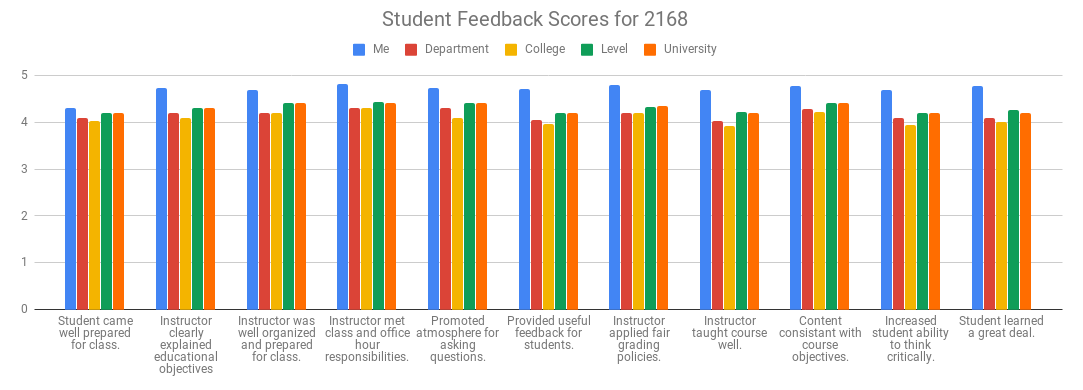
\includegraphics[width=1\linewidth]{2168SFF}
	\caption{My averaged student feedback for Data Structures. }
	\label{fig:2168sff}
\end{figure}


\begin{figure}
	\centering
	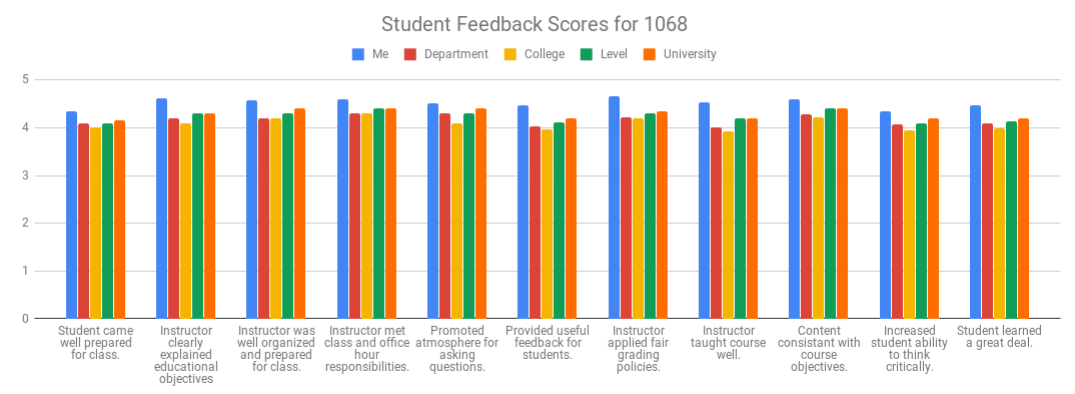
\includegraphics[width=1\linewidth]{1068SFF}
	\caption{My averaged student feedback for Program Design \& Abstraction.}
	\label{fig:1068sff}
\end{figure}




\begin{figure}
	\centering
	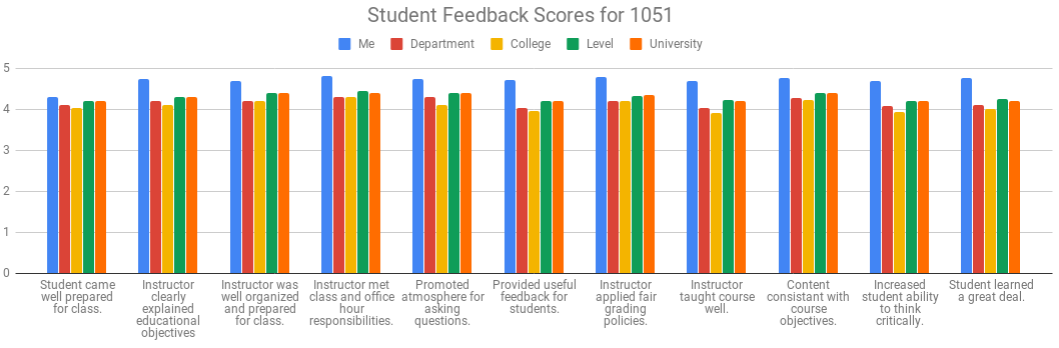
\includegraphics[width=1\linewidth]{1051SFF}
	\caption{My averaged student feedback for Introduction to Problem Solving and Programming in Python.}
	\label{fig:1051sff}
\end{figure}



My full student feedback forms can be found in the included documents.
\subsection{Student SFF Excerpts}
My comments left by students have been overwhelmingly positive and can be found in the student feedback forms.
I've included some choice examples (misspellings and grammar are unaltered):

\subsubsection*{Responses to ``What aspects of the course or the instructor’s approach contributed most to your learning''?}

\begin{small}
	
\begin{quotation}
	Flipped lectures are a fabulous idea for a programming class. A student can spend their own time out of class reviewing the material necessary for the upcoming assignment and then ask any and all questions to the professor in class. This avoids the constant struggle in a programming class of not being able to find the error in your code the night before the lab is due.
\end{quotation}

\begin{quotation}
	Good sense of humor, more enthusiasm than youd expect from a married guy with a baby in the morning, overall energetic personality that gave life to the class. Also straightforward lectures that were recorded to make it easy for anyone who missed class or needed a reminder on certain things.
\end{quotation}

\begin{quote}
	 I loved the flipped classroom style he used. Quizzes were fair, if on the easy side. Overall I felt like material covered was pretty simple, and could have been more aggressive in difficulty, but Rosen particularly did a good job of clarifying common tripping points, and made effort to individualize his approach per student. Clearly he has a desire to teach, and isnt just a professor by mandate. Incredible man
	
\end{quote}

\begin{quotation}
	
	Rosen was an awesome professor and is clearly very passionate about data structures. Very helpful when questions were asked. Also speaks volumes about him that he had a newborn kid during the earlier weeks of class, and was still very present!
	
\end{quotation}
	
	
\begin{quotation}
	Professor Rosen has a unique ability to make a two and a half hour class not drag by. His insights into the way data structures fundamentally work is what really makes him an excellent professor.
	
\end{quotation}


\begin{quotation}
	Rosen is the man. Explains clearly and is PATIENT with students as they learn. A lot of professors struggle with this. Encouraging and nice guy.
\end{quotation}

\begin{quotation}
	Dear CIS department, GET MORE PROFESSORS LIKE ANDREW ROSEN. I actually felt encouraged in the class to learn because he laid the material out as simply as he could. [\textellipsis]\footnote{I removed a remark about another Professor.} I did not feel like I had to come into class with a whole lot of knowledge in order to succeed. He gave examples, hints and spent time explaining each topic to us.  Also his pratice tests, reviews of the pratice test, use of slides and recordings of the class were extremely helpful. I honestly appreciate this teacher.
	
\end{quotation}

\begin{quotation}
	It was very clear hes thought a lot about how to teach this course. This was clear in the ways he sometimes defied teaching convention in thoughtful ways. For example, the requirement for students to demonstrate their code to him or the TA, his insistence that we learn how to use libraries on our own, and any other numerous example (some of which were very subtle.) Thats not to mention the fact that his wife had a baby the second day of the course, and yet he was always there for lab hours. Dr. Andrew Rosen deeply impressed me. He may very well be the most skilled teacher Ive ever had.
	
\end{quotation}

\begin{quotation}
	Professor Rosen is the best teacher Ive had at Temple, and its not even close. He really enjoyed the teaching and I think the enthusiasm showed, without being over the top and annoying. He is the most organized teacher. We knew exactly where we were on relation to the totality of the class. He answered every question, and I mean every question, without ever getting annoyed.he recorded the class, which I still why every doesnt do it. Even the little things, he always made sure he was in view of the camera when he wrote on the board. He writes his own test questions, or at the very least selected questions that sounded like he wouldve wrote them, which during the stress of a test im already used to the meaning which rereading 50 times. He was extremely fair but not a pushover. His tests werent easy but I felt very prepared. He is an amazing and I hope Im able taught by him again.
	
\end{quotation}

\begin{quotation}
	The homeworks were often difficult in a good way. On an unrelated side note, Dr. Rosen is hilarious and I always enjoyed going to Class.
\end{quotation}

\end{small}


Whilst I am skeptical of student's attribution of being super organized (a quality I think many of those reading this document would be horrified to have applied to them as well.  The students rarely see the ``sausage'' of a course being made), these quotations highlight many of the aspects that I cultivate in my classroom.  


I record my lectures so my students can peruse them at their convenience and review the content whenever they need it.  
My students know that I am always available for them; if I can't meet them on campus during normal work hours, they know that they can reach out and meet me using video chat in the evening.
They also know that I understand how difficult learning to program is, and that I'll be patient with them and work with them to understand the material.
My students can be kept engaged in the classroom, even if the lecture period is ridiculously long, because I try to incorporate many varieties of active learning in my class.



\section{Curriculum Development}
I am heavily involved in the curriculum development and coordination for the department.
I have written all the exams for my sections and write the common final exam for CIS 2168. 
I develop interesting and engaging assignments for our students, such as my maze solving program, where students are given a randomly generated maze and have to write a program to color the path to the exit, and find and adapt interesting assignments for our students to work on.

I coordinate the content of my courses with Professor Fiore, who currently teaches the majority of the sections of CIS 1068, and Professor Hughes, who teaches CIS 3223 - Data Structures and Algorithms.
CIS 1051 serves as a prerequisite for CIS 1068, so I work with Professor Fiore to make sure we don't repeat assignments, create similar questions to track student knowledge retention, and make sure CIS 1051 students are prepared for CIS 1068.  Similarly, CIS 1068 serves as the prerequisite to CIS 2168, so we work to make sure that we can again track student knowledge retention over courses and that students coming out of CIS 1068 are prepared for CIS 2168.  
CIS 2168 is a prerequisite to CIS 3223, so I coordinate with Professor Hughes so that he knows what to expect of our students knowledge and experience, which prevents us from wasting time covering the same topic in multiple courses.



I have also created a new course, CIS 5016, Data Structures and Objects, a graduate level accelerated introduction to computer science and data structures.
This course is being taught online, which is one of the most exciting developments in our department.
Creating this course with the Office of Digital Education has required a tremendous amount of work.  
I've had to create numerous modules plans with learning objective, as well as scripts with visual instructions for our videos at extremely accelerated pace, as we had to create the course in half the time normally allotted for creation.

The end result is an extremely polished online experience for our students with videos that are comparable to the best quality videos that can be found online.\footnote{If you have not looked at the linked video at \url{https://player.vimeo.com/video/313364524} yet, I strongly urge you to do so, so you can get an idea of the amount of professionalism and high quality we are bringing to the course.} 
I've developed the content for this course in such a way that we can also feed many of the videos and quizzes that have been made for this class into our undergraduate CIS 1068 and CIS 2168 courses, so that they can take advantage of this high-end material too.

Because I am one of the professors taken the lead in the initiative of developing online courses, I am currently engaged to mentor my fellow faculty members on how to build their own online course, how to maintain and run their courses, and how to write and record their own content,

\section{Recordings and Flipped Lectures}

I record all of my lectures and upload them to \url{https://www.youtube.com/channel/professorrosen}, my YouTube channel.\footnote{I use YouTube as I know it's a reliable service that students can access from any device without any hassle.}  
I started recording my lectures during my first semester at Temple, as one of my courses was intended to be offered simultaneously on the Japan campus.  My lectures would be recorded and later watched by the students at Temple's Japan campus, where they would then do the work on their own.\footnote{Experiences with this setup is a part of what drove me to offer the classes in person on the Japan campus.}
I realized there was no reason not to provide these lectures to all my students.
The student response, as you have seen, has been overwhelmingly positive.

Recording all my lectures, in addition to uploading all my code from class, allows students to focus on the content and concepts that I am putting on the screen, rather than trying to get down everything I do and say verbatim.
It removes the anxiety from a student who zones out for a few minutes, wondering what horrors are now forthcoming after I have uttered the phrase ``and you should really study this.''
Sick students don't drag themselves to class and infect their peers while they struggle to take down notes, they know they can review the material later at their leisure.
Exams become less stressful as students know they can review the material exactly as I presented it to them in class.

My student continually tell me how useful my recordings are to their success in my course.  In fact, I get thanked at least once a semester by a student who has never been in any of my courses, saying that my videos helped them succeed in another professor's section.

%I began by using the Panopto system provided by the College of Science and Technology, but eventually switched to using OBS due to the customization it provides along with the more granular control over what I can capture. 



\subsection{Live Coding}
The bulk of my traditional lectures are comprised of live-coding.
Live-coding is where you create and run the example code in front of the students, and I have used it in most of my lectures.
By programming in class and prompting students for input, I am able to use the lecture time to get students coding, albeit vicariously.
It makes programming feel more real and less theoretical.

Live-coding means making mistakes, and these mistakes, intentional or unintentional, help students become accustomed to the debugging process they will have to do themselves.
In addition, seeing an ostensible expert make mistakes and correct them makes coding much less intimidating and helps mitigate the feeling of impostor syndrome that so often affects students with no prior exposure to programming.
%\subsubsection{Demoing}
%I do know any professors who look forward to grading a giant pile of student work, and grading programs is particularly tedious, as program and project structure can differ wildly from. 
%


\subsection{Flipped Course}
The idea of a flipped classroom for programming classes seemed like a natural fit and  a clear evolution from recording my lectures.  
The \textit{only} way to learn programming is by actually getting your hands dirty and trying to solve a problem, making and correcting innumerable mistakes along to way.  
I often tell my class the only reason I can debug a problem  they have  in just a few sections is that I've made that same mistake about 50 times and they just made that mistake for the first time.

But that first time, as they say, is a doozy.  
I know from both personal experience  and student feedback that the first time you encounter some errors they can take hours to solve, if not longer.  
The mistake can  something utterly trivial, such as using an ``l'' where an ``I'' should be, or just forgetting to call the piece of code you just wrote.
These mistakes are human and you feel dumb and inadequate when you figure out the simple think that just ate up three hours.
It's not an enjoyable experience for programmers and its a common one.  
It shouldn't have to be as painful as it is.

Flipping a course turns it on its head.  
Students watch prerecorded content before coming to class for the week, then they do active learning exercises in class and take quizzes.  The rest of the time in the lecture is made available for the students to do their homework assignments.  Here, they make same mistakes any beginner makes, but the difference is I am here to immediately fix it or guide them in the right direction before they get too off track.


But more importantly, it gives me the one on one time with students that is just so lacking in a traditional lecture.  
I get to meet with them and address their individual needs.
Are they having trouble with a particular topic? I can spend a few minutes sitting down with the student and personally explaining it to them.  Are students nearby listening in?  I can address the whole class for a bt and give some good examples and pointers.  Does the student need a bigger challenge? I know ways to make most projects more exciting, or I can pass the student an alternate assignment, or I can pair the student with one who is struggling.

Flipping the course was a lot of upfront work.  
I had to record about an hour and a half to two hours of material every week, which took about twice as long to do that actually recording due to numerous retakes.
However, now that the upfront work has been done, the course runs extremely smoothly and I can update individual videos on an ad-hoc basis.

Each video is somewhere between five to twenty minutes, depending on the topic, and each video covers a discrete, specific aspect of the course.
This allows the students to watch a video that is short enough to help mitigate distraction, as well as making reviewing the material easier, as they can quickly travel to the content they want to review.

%
%\section{Japan}
%One 


%
\section{Conclusion}
Teaching is my passion and I devote myself to it.
I create new courses, I make amazing content for the courses we currently, I help my students whenever they need it, and I introduce novel teaching techniques and paradigms into my courses to provide my students with better outcomes.
My students have both quantitatively and qualitatively shown that they find my teaching exceptional.
The college has found my work to be exceptional when I was bestowed the Dean's Distinguished Teaching Award.
I am grateful to be a member of institution that acknowledges and rewards its faculty for its accomplishments in teaching and plan on continuing to create even better experiences and outcomes for our students.

\end{document}
